% SVN info for this file
\svnidlong
{$HeadURL$}
{$LastChangedDate$}
{$LastChangedRevision$}
{$LastChangedBy$}

\chapter{Serie di funzioni}
\labelChapter{seriefunzioni}

\begin{introduction}
	‘‘BEEP BOOP QUESTA È UNA CITAZIONE.''
\begin{flushright}
	\textsc{Marinobot,} dopo aver finito le citazioni stupide.
\end{flushright}
\end{introduction}
\lettrine[findent=1pt, nindent=0pt]{L}{e} Nel \refChapter{convergenzafunzioni} abbiamo iniziato a trattare la convergenza uniforme e puntuale di successioni di funzioni. Adesso passiamo a parlare di serie di funzioni.
\textbf{[COMPLETARE]} % TO DO: completare l'intro
\section{Serie in uno spazio normato}
Innanzitutto, ricordiamo le definizioni di serie a valori reali e di convergenza (assoluta) di una serie a valore reali.
\begin{define}[Serie a valori reali e convergenza di una serie.]~{}\\
	Data una successione $x_n\in\realset$, $n\geq 0$, la \textbf{serie}\index{serie} $\displaystyle\sum_{k=0}^{+\infty}x_k$ è la somma di tutti gli elementi della successione.\\
	Considerata la \textit{somma parziale}, o altresì detta \textbf{ridotta}\index{ridotta}
	\begin{equation}
		s_n=\sum_{k=0}^{n}x_k\quad\forall n\geq 0
	\end{equation}
si dice che la serie $\displaystyle\sum_{k=0}^{+\infty}x_k$ \textbf{converge}\index{convergenza!di una serie}\seeonlyindex{convergenza!di una serie}{convergenza!semplice} se converge la successione $s_n$; si pone in tal caso
\begin{equation}
	\sum_{k=0}^{+\infty}x_k=\lim_{n\to+\infty}s_n
\end{equation}
\end{define}
\begin{define}[Convergenza assoluta.]~{}\\
	Sia $x_n$ una successione a valori reali. La serie $\displaystyle\sum_{k=0}^{+\infty}x_k$ \textbf{converge assolutamente}\seeonlyindex{convergenza!totale}{convergenza!assoluta} in $\realset$ se converge la serie $\displaystyle\sum_{k=0}^{+\infty}\abs{x_k}$.
\end{define}
\begin{theorema}[Convergenza assoluta implica convergenza semplice.]~{}\\\label{teoremaassimplicasemplice}
	Ogni serie di numeri reali assolutamente convergente è anche semplicemente convergente.
\end{theorema}
\begin{demonstration}
	Per dimostrare che la serie $\displaystyle\sum_{k=0}^{+\infty}x_k$ converge, per il \textit{Criterio di Cauchy per le serie}\footnote{Nelle ‘‘Note aggiuntive'', a pagina XXX è possibile trovare maggiori dettagli sul criterio di Cauchy.} è sufficiente provare che
	\begin{equation*}
		\forall \epsilon>0\ \exists N\in\naturalset\colon\forall n\geq N,\ \forall p\in\naturalset\ \abs{x_{n+1}+x_{n+2}+\ldots+x_{n+p}}<\epsilon
	\end{equation*}
	Per ipotesi la serie $\displaystyle\sum_{k=0}^{+\infty}\abs{x_k}$ converge: per il Criterio di Cauchy, si ha
	\begin{equation*}
		\forall \epsilon>0\ \exists N\in\naturalset\colon\forall n\geq N,\ \forall p\in\naturalset\ \abs{\abs{x_{n+1}}+\abs{x_{n+2}}+\ldots+\abs{x_{n+p}}}=\abs{x_{n+1}}+\abs{x_{n+2}}+\ldots+\abs{x_{n+p}}<\epsilon
	\end{equation*}
	D’altra parte, dalla disuguaglianza triangolare segue che
	\begin{equation*}
		\abs{x_{n+1}+x_{n+2}+\ldots+x_{n+p}}<\abs{x_{n+1}}+\abs{x_{n+2}}+\ldots+\abs{x_{n+p}}<\epsilon,\ \forall n\in\naturalset,\ \forall p\in\naturalset
	\end{equation*}
Dalle ultime due relazioni si deduce immediatamente la prima relazione e dunque la tesi.
\end{demonstration}
\begin{observe}\label{convergenzaassolutadipendedacauchy}
	Il teorema appena dimostrato è una conseguenza della \textbf{completezza} di $\realset$. Infatti, abbiamo usato il \textit{criterio di Cauchy}, che si basa sul fatto che le successioni di Cauchy convergono sempre in $\realset$ e quindi proprio per la completezza dei reali.
\end{observe}
Il viceversa del teorema appena dimostrato non è valido, come segue dal seguente controesempio.
\begin{example}
	Consideriamo la serie $\displaystyle\sum_{n=1}^{+\infty}\left(-1\right)^n\frac{1}{n}$: non converge assolutamente in quanto la serie, con gli elementi in modulo, diventa
	\begin{equation*}
		\sum_{n=1}^{+\infty}\abs{\left(-1\right)^n\frac{1}{n}}=\sum_{n=1}^{+\infty}\frac{1}{n}
	\end{equation*}
	che, essendo la \textbf{serie armonica}\footnote{Nelle ‘‘Note aggiuntive'', a pagina XXX è possibile trovare maggiori dettagli sulle serie notevoli.}, non converge. Tuttavia, la serie semplice è una serie a segni alterni e poiché
	\begin{itemize}
		\item $\frac{1}{n}$ è decrescente $\forall n\geq 1$.
		\item $\displaystyle\lim_{n\to+\infty}\frac{1}{n}=0$.
	\end{itemize} 
	per il \textit{criterio di Leibniz} la serie semplice converge. Pertanto, la convergenza semplice non implica la convergenza assoluta.
\end{example}
Prendiamo ora $x_n\in X$, con $X$ un insieme generico. Per generalizzare la definizione di serie convergente abbiamo bisogno che su $X$ si possano compiere i seguenti passaggi:
\begin{itemize}
	\item Poter definire $s_n$, cioè è necessario \textit{sommare} elementi di $X$.
	\item Poter definire la \textit{convergenza} in $X$.
\end{itemize}
Se dotiamo l'insieme $X$ di una struttura di \textbf{spazio normato} possiamo generalizzare ad una serie generale le definizioni precedentemente enunciate per le serie a valori reali: infatti, se $X$ è spazio normato gode sia dell'essere uno spazio metrico (e quindi è spazio topologico di Hausdorff, il che permette di definire univocamente la convergenza della successione) sia dell'essere spazio vettoriale (che permette la somma di elementi).\\
\begin{define}[Serie e convergenza di una serie.]~{}\\
	Data una successione $x_n\in X$ spazio \textit{normato}, $n\geq 0$, la \textbf{serie}\index{serie} $\displaystyle\sum_{k=0}^{+\infty}x_k$ è la somma di tutti gli elementi della successione.\\
	Considerata la \textit{somma parziale}, o altresì detta \textbf{ridotta}\index{ridotta}
	\begin{equation}
		s_n=\sum_{k=0}^{n}x_k\quad\forall n\geq 0
	\end{equation}
	si dice che la serie $\displaystyle\sum_{k=0}^{+\infty}x_k$ \textbf{converge}\index{convergenza!di una serie}\seeonlyindex{convergenza!di una serie}{convergenza!semplice} se converge la successione $s_n$; si pone in tal caso
	\begin{equation}
		\sum_{k=0}^{+\infty}x_k=\lim_{n\to+\infty}s_n
	\end{equation}
\end{define}
\begin{define}[Convergenza totale o assoluta.]~{}\\
	Sia $\left(X,\norm{\cdot}\right)$ spazio normato e $x_n$ una successione in $X$. La serie $\displaystyle\sum_{k=0}^{+\infty}x_k$ \textbf{converge totalmente}\index{convergenza!totale} o \textbf{assolutamente}\seeonlyindex{convergenza!totale}{convergenza!assoluta} in $X$ se converge la serie $\displaystyle\sum_{k=0}^{+\infty}\norm{x_k}$.
\end{define}
Dall'osservazione a pag. \pageref{convergenzaassolutadipendedacauchy} il teorema ‘‘Convergenza assoluta implica convergenza semplice'' (teorema \ref{teoremaassimplicasemplice}, pag. \pageref{teoremaassimplicasemplice}) necessita della \textit{completezza} dei reali. Per generalizzarlo ci basta lavorare in \textit{spazi normati completi}.
\begin{theorema}[Convergenza totale o assoluta implica convergenza semplice.]~{}\\
	Ogni serie in $X$ spazio normato completo totalmente convergente è anche semplicemente convergente.
\end{theorema}
\begin{demonstration}
	La dimostrazione è analoga a quella affrontata nel teorema  \ref{teoremaassimplicasemplice}, pag. \pageref{teoremaassimplicasemplice}: è sufficiente sostituire al valore assoluto $\abs{\cdot}$ la norma $\norm{\cdot}$.
\end{demonstration}
In generale, il problema della convergenza in spazi normati è \textit{inesplorato}, ma se lo spazio è \textit{completo} possiamo passare per la \textit{convergenza totale} e studiare una serie a valori reali tramite i \textit{criteri di convergenza}\footnote{Nelle ‘‘Note aggiuntive'', a pagina XXX è possibile trovare maggiori dettagli sui criteri di convergenza delle serie a valori reali.} noti dall'\textsc{Analisi 1}.\\
\section{Serie di funzioni}
Consideriamo lo spazio  $X=\mathcal{C}\left(\left[a,b\right];\ \realset\right)=\mathcal{C}\left(\left[a,b\right]\right)$ delle funzioni continue su un intervallo compatto con la \textit{metrica lagrangiana}:
\begin{equation*}
	\mvf{d}{f}{g}=\max_{x\in\left[a,b\right]}\abs{f\left(x\right)-g\left(x\right)}
\end{equation*}
Una serie convergente $\displaystyle\sum_{k=0}^{+\infty}f_k$ in questo spazio si può quindi scrivere, per definizione, come
\begin{equation*}
	\sum_{k=0}^{+\infty}f_k=\lim_{n\to+\infty}\sum_{k=0}^{n}f_k=\lim_{n\to+\infty}S_n
\end{equation*}
dove $S_n$ è una successione di funzioni. Allora la condizione di convergenza di serie in $X$ si può formulare come
\begin{equation*}
	\sum_{k=0}^{+\infty}f_k\text{ converge in }\mathcal{C}\left(\left[a,b\right]\right)\iff S_n\text{ converge con metrica lagriangiana in}\mathcal{C}\left(\left[a,b\right]\right)
\end{equation*}
ossia
\begin{equation*}
	\sum_{k=0}^{+\infty}f_k\text{ converge in }\mathcal{C}\left(\left[a,b\right]\right)\iff S_n\text{ converge uniformemente in}\mathcal{C}\left(\left[a,b\right]\right)
\end{equation*}
Per la stessa osservazione fatte a pag. \pageref{convergenzalagrangianaeuniforme}, sezione \ref{convergenzalagrangianaeuniforme}, per parlare di convergenza uniforme non sono necessarie né la \textit{compattezza} di $\left[a,b\right]$ né la \textit{continuità} delle funzioni.\\
Possiamo \textit{estendere} la definizione di convergenza di una serie di funzioni per
\begin{equation*}
	\funz{f_n}{A\subseteq \realset}{\realset}
\end{equation*}
con $A$ insieme contenuto nei reali o, ancora più in generale, per funzioni del tipo
\begin{equation*}
	\funz{f_n}{X}{Y}
\end{equation*}
dove $X$ è un \textit{insieme qualunque} e $Y$ è uno \textbf{spazio normato completo}.\\
Studieremo quindi le \textbf{serie di funzioni}\index{serie!di funzioni} $\displaystyle\sum_{k=0}^{+\infty}f_k\left(x\right)$; per studiare la \textit{convergenza} di tali serie applicheremo le convergenze viste in precedenza alla \textit{successione delle ridotte} $\displaystyle S_n\left(x\right)=\sum_{k=0}^{n}f_k\left(x\right)$.
\begin{define}[Convergenza di una serie di funzioni.]~{}\\
	\begin{itemize}
		\item \textbf{(CP)} La serie $\displaystyle\sum_{k=0}^{+\infty}f_k\left(x\right)$ \textbf{converge puntualmente} in $x\in A$ se $S_n\left(x\right)$ converge puntualmente in $x\in A$.
		\item \textbf{(CU)} La serie $\displaystyle\sum_{k=0}^{+\infty}f_k\left(x\right)$ \textbf{converge uniformemente} in $x\in A$ se $S_n\left(x\right)$ converge uniformemente su $A$.
	\end{itemize}
\end{define}
\subsection{Il criterio di Weierstrass}
Per motivi che saranno chiari a partire dalla sezione \ref{seriedipotenze} (pag. \pageref{seriedipotenze}) sulle serie di potenze, in questa sottosezione lavoreremo nello spazio dei complessi $\complexset$.\\
Abbiamo dato la definizione di convergenza uniforme di una serie di funzione, ma essa non è di facile applicazione operativa. Infatti, la serie $\displaystyle\sum_{n=0}^{+\infty}f_n\left(z\right)$ converge uniformemente su $A\subseteq\complexset$ se e solo se, definita $S\left(z\right)$ la funzione limite delle ridotte $\displaystyle S_n\left(z\right)=\sum_{k=0}^{n}f_k\left(z\right)$, vale
\begin{equation*}
	\lim_{n\to+\infty}\left(\sup_{z\in A}\abs{S_n\left(z\right)-S\left(z\right)}\right)=0
\end{equation*}
Tuttavia, questa funzione richiede la conoscenza della \textit{somma} $S\left(z\right)$, cosa che in generale \textit{non} avviene. Usare direttamente il criterio di Cauchy per la convergenza uniforme è sicuramente più conveniente, ma non è semplice comunque da verificare. Esiste tuttavia una condizione \textit{sufficiente} che consente di provare la convergenza uniforme senza la conoscenza della somma limite.
\begin{proposition}[Criterio di Weierstrass.]~{}\\\label{criteriodiweierstrass}
	Siano $\funz{f_n}{A\subseteq \complexset}{\complexset}$ tale che
	\begin{enumerate}
		\item $\forall n\ \exists c_n\in\realset\colon\ \abs{f_n\left(z\right)}\leq c_n,\ \forall z\in A$.
		\item $\displaystyle\sum_{n=1}^{+\infty}c_n$ converge.
	\end{enumerate}
Allora $\displaystyle\sum_{n=1}^{+\infty}f_n\left(z\right)$ converge uniformemente in $A$.
\end{proposition}
\begin{observe}
	La dimostrazione utilizza il criterio di Cauchy per la convergenza uniforme.
\end{observe}
\begin{observe}\textsc{Significato del criterio.}\\
	Le ipotesi $1)$ e $2)$ implicano immediatamente la convergenza puntuale della serie di potenze in ogni $z\in A$. Infatti, fissato $z$ ho la relazione $\abs{f_n\left(z\right)}\leq c_n$; da questo vale
	\begin{equation*}
		\sum_{n=0}^{+\infty}\abs{f_n\left(z\right)}\leq \sum_{n=0}^{+\infty}c_n
	\end{equation*}
e, poiché la serie $\displaystyle\sum_{n=0}^{+\infty}c_n$ converge, $\displaystyle\sum_{n=0}^{+\infty}\abs{f_n\left(z\right)}$ converge per criterio del confronto e quindi la serie di funzioni converge puntualmente.\\
Quello che osserviamo nello specifico è che l'ipotesi $1)$ funge da \textit{maggiorazione uniforme} della serie di funzioni su $A$, da cui possiamo ricavare, anche a partire dalla convergenza puntuale della serie, la convergenza uniforme su $A$.
\end{observe}
\section{Proprietà di regolarità di una serie di funzioni}
Ci poniamo ora il problema di studiare come si modificano i teoremi di \textit{limitatezza}, \textit{continuità}, \textit{integrabilità}, \textit{integrabilità} e \textit{derivabilità} visti nel \refChapter{convergenzafunzioni} nel caso delle \textit{serie di funzioni}.
\subsection{Limitatezza}
\begin{theorema}[Teorema di limitatezza per serie.]~{}\\
	Siano $\displaystyle \funz{f_n}{A\subseteq\realset}{\realset},\ n\geq 1$ tali che
	\begin{enumerate}
		\item $f_n$ limitata su $A,\ \forall n\geq 1$.
		\item $\displaystyle\sum_{n=0}^{+\infty}f_n$ converge \textit{uniformemente} a $f$ su $A$.
	\end{enumerate}
	Allora, posto $\displaystyle S\left(x\right)=\sum_{n=0}^{+\infty}f_n,\ \forall x\in A$, $S\left(x\right)$ è limitata su $A$.
\end{theorema}
\begin{demonstration}
	Posto $\displaystyle S_n\left(x\right)=\sum_{k=0}^{n}f_k\left(x\right),\ \forall x\in A$, allora si ha:
	\begin{itemize}
		\item $S_n$ limitata su $A$, poiché le $f_k$ lo sono.
		\item $S_n$ convergente uniformemente a $S$ su $A$.
	\end{itemize}
	Per il teorema di limitatezza per le successioni, $S$ è limitata su $A$.
\end{demonstration}
\subsection{Continuità}
\begin{theorema}[Teorema di continuità per serie.]~{}\\
	Siano $\funz{f_n}{A\subseteq\realset}{\realset},\ n\geq 1$ tali che
	\begin{enumerate}
		\item $f_n$ continua su $A,\ \forall n\geq 1$.
		\item $\displaystyle\sum_{n=0}^{+\infty}f_n$ converge \textit{uniformemente} a $f$ su $A$.
	\end{enumerate}
	Allora, posto $\displaystyle S\left(x\right)=\sum_{n=0}^{+\infty}f_n,\ \forall x\in A$, $S\left(x\right)$ è continua su $A$.
\end{theorema}
\begin{demonstration}
	Posto $\displaystyle S_n\left(x\right)=\sum_{k=0}^{n}f_k\left(x\right),\ \forall x\in A$, allora si ha:
	\begin{itemize}
		\item $S_n$ continua su $A$, poiché le $f_k$ lo sono.
		\item $S_n$ convergente uniformemente a $S$ su $A$.
	\end{itemize}
	Per il teorema di continuità per le successioni, $S$ è continua su $A$.
\end{demonstration}
\subsection{Integrabilità e scambio tra integrale e serie}
\begin{theorema}[Teorema di integrabilità per serie, scambio tra integrale e serie.]~{}\\
	Sia $\funz{f_n,f}{\left[a,b\right]}{\realset},\ n\geq 1$ tali che
	\begin{enumerate}
		\item $f_n\in\mathcal{R}\left(\left[a,b\right]\right),\ \forall n\geq 1$.
		\item $\displaystyle\sum_{n=0}^{+\infty}f_n$ converge \textit{uniformemente} a $f$ su $\left[a,b\right]$.
	\end{enumerate}
	Allora, posto $\displaystyle S\left(x\right)=\sum_{n=0}^{+\infty}f_n,\ \forall x\in \left[a,b\right]$:
	\begin{enumerate}
		\item $S\in\mathcal{R}\left(\left[a,b\right]\right)$.
		\item Vale lo \textbf{scambio tra integrale e serie}\index{scambio tra integrale e serie}:
		\begin{equation}
			\int_{a}^{b}\sum_{k=0}^{+\infty}f_k\left(x\right)dx=\sum_{k=0}^{+\infty}\int_{a}^{b}f_k\left(x\right)dx
		\end{equation}
	\end{enumerate}
\end{theorema}
\begin{demonstration}
	Posto $\displaystyle S_n\left(x\right)=\sum_{k=0}^{n}f_k\left(x\right),\ \forall x\in \left[a,b\right]$, allora si ha:
	\begin{itemize}
		\item $S_n\in\mathcal{R}\left(\left[a,b\right]\right)$, poiché le $f_k$ lo sono.
		\item $S_n$ convergente \textit{uniformemente} a $S$ su $\left[a,b\right]$.
	\end{itemize}
	Per il teorema di integrabilità per le successioni:
	\begin{itemize}
		\item $S\in\mathcal{R}\left(\left[a,b\right]\right)$.
		\item Vale il \textit{passaggio al limite sotto segno di integrale} per la successione delle ridotte, ossia
		\begin{equation*}
			\lim_{n\to+\infty}\int_{a}^{b}S_n\left(x\right)dx=\int_{a}^{b}S\left(x\right)dx
		\end{equation*}
		Poiché l'\textit{integrale di una somma finita} è uguale ad una \textit{somma finita di integrali}, il primo membro dell'equazione può essere riscritto come
		\begin{equation*}
			\lim_{n\to+\infty}\int_{a}^{b}\sum_{k=0}^{n}f_k\left(x\right)dx=\lim_{n\to+\infty}\sum_{k=0}^{n}\int_{a}^{b}f_k\left(x\right)dx=\sum_{k=0}^{+\infty}\int_{a}^{b}f_k\left(x\right)dx
		\end{equation*}
		e poiché $\displaystyle \int_{a}^{b}S\left(x\right)dx=\int_{a}^{b}\sum_{k=0}^{+\infty}f_k\left(x\right)dx$, otteniamo la tesi:
		\begin{equation*}
			\int_{a}^{b}\sum_{k=0}^{+\infty}f_k\left(x\right)dx=\sum_{k=0}^{+\infty}\int_{a}^{b}f_k\left(x\right)dx
		\end{equation*}
	\end{itemize}
\end{demonstration}
\section{Serie di potenze}\label{seriedipotenze}
\begin{define}
	Una \textbf{serie di potenze}\index{serie!di potenze} è una serie di funzioni della forma
	\begin{equation}
		\sum_{n=0}^{+\infty}a_n	\left(x-x_0\right)^n
	\end{equation}
	con $a_n$ numeri reali (eventualmente dipendenti da $n$) e $x,\ x_0\in A\subseteq\realset$, dove $x_0$ è dato.
\end{define}
L'ambito naturale di studio delle serie di potenze è $\complexset$: da qui in poi considereremo la serie (con anche i suoi coefficienti) in campo complesso:
\begin{equation}
	\sum_{n=0}^{+\infty}a_n	\left(z-z_0\right)^n\qquad a_n,\ z\in\complexset
\end{equation}
dove $z\in A\subseteq\complexset$. Cambiando le variabili possiamo centrare la serie in $z_0=0$, cioè studiare la serie
\begin{equation}
	\sum_{n=0}^{+\infty}a_nz^n=a_0+a_1z+a_2z^2+a_3z^3\ldots
\end{equation}
Chiaramente la serie così scritta converge in $z=0$ (o, se prendiamo la serie \textit{non} centrata nell'origine, in $z=z_0$), dato che la serie ha termini \textit{costantemente nulli} e quindi è banalmente convergente.\\
Ci interessa ora studiare in quale insieme di $\complexset$ tali serie convergono. 
\begin{theorema}[Insieme di convergenza.]~{}\\\label{insiemediconvergenza}
	Se una serie di potenze converge in $z_0\in\complexset$, allora essa converge (assolutamente) in ogni punto $z$ con $\abs{z}<\abs{z_0}$.
\end{theorema}
\begin{demonstration}
	Sappiamo dalle ipotesi che la serie $\displaystyle\sum_{n=0}^{+\infty}a_nz_0^n$ è convergente, quindi per la condizione necessaria di convergenza il termine $a_nz_0^n$ tende a zero. Per definizione di limite significa che
	\begin{equation*}
		\forall \epsilon >0\ \exists N=N\left(\epsilon\right)\in\naturalset\colon\forall n\geq N\ \abs{a_nz_0^n}<\epsilon
	\end{equation*}
	Scegliamo arbitrariamente $\epsilon = 1$, cioè $\exists N_1=N\left(1\right)\colon \forall n\geq N$ vale $\abs{a_nz_0^n}<1$.
	Allora definitivamente vale
	\begin{equation*}
		\abs{a_nz^n}=\abs{a_nz_0^n}\abs{\frac{z}{z_0}}^n\leq\abs{\frac{z}{z_0}}^n
	\end{equation*}
Poiché per ipotesi $\abs{z}<\abs{z_0}$, vale $\abs{\frac{z}{z_0}}<1$ e quindi la serie geometrica $\displaystyle\sum_{n=0}^{+\infty}\abs{\frac{z}{z_0}}$ converge. Per il teorema di confronto segue che anche la serie $\displaystyle\sum_{n=0}^{+\infty}\abs{a_nz^n}$ è convergente e quindi $\displaystyle\sum_{n=0}^{+\infty}a_nz^n$ converge (assolutamente).
\end{demonstration}
Con questo non solo abbiamo dimostrato che se la serie di potenze converge in $z_0$ la serie converge in tutti i punti $z$ con $\abs{z}<\abs{z_0}$, ma implicitamente sappiamo anche che la serie \textit{non} converge in $z_0$ allora \textit{non} converge per $\abs{z}>\abs{z_0}$.\\
Infatti, se in $z_0$ la serie non converge supponiamo per assurdo che esista $z^\ast$, con $\abs{z^\ast}>\abs{z_0}$, in cui la serie converge. Per il teorema appena dimostrato in tutti i punti $z$ con $\abs{z}<\abs{z^\ast}$ la serie di potenze converge, ma fra questi è compreso anche $z_0$ dove essa \textit{non} converge.
\subsection{Il raggio di convergenza}
Per queste osservazioni l'insieme di convergenza della serie è un \textit{cerchio} centrato nell'origine di un certo \textit{raggio} $R$. Diamo una definizione formale di questo raggio.
\begin{define}[Cerchio e raggio di convergenza.]~{}\\
	Preso $\displaystyle A=\left\{z\mid\sum_{n=0}^{+\infty} a_n z^n \ \mbox{converge} \right\}\subseteq \complexset$ l'insieme di convergenza della serie di potenze centrata in $z_0=0$ e consideriamo l'insieme $E=\left\{\abs{z}\mid z\in A\right\}\subseteq\realset$ dato da tutti i moduli dei punti di convergenza della serie. Il \textbf{raggio di convergenza}\index{raggio di convergenza} è definito come
	\begin{equation*}
		r\coloneqq\sup E
	\end{equation*}
Esso può essere:
\begin{itemize}
	\item $R=0$; in tal caso la serie converge \textit{solo} per $z=0$.
	\item $R=+\infty$; in tal caso la serie converge \textit{per ogni} $z\in\complexset$.
	\item $0<R<+\infty$; in base al teorema \ref{insiemediconvergenza}, pag. \ref{insiemediconvergenza}, la serie converge (assolutamente) per $\abs{z}<r$, \textit{non} converge per $\abs{z}<r$ e a priori non abbiamo \textit{alcuna informazione} per i punti $z$ sul \textit{bordo}, cioè tali che $\abs{z}=r$. L'\textit{insieme di convergenza} risulta essere un \textbf{cerchio aperto}\index{cerchio di convergenza} centrato nell'origine di raggio $R$, a cui si aggiungono eventualmente altri punti di convergenza sul \textit{bordo} (tutti, nessuno o solo alcuni).
\end{itemize}
\end{define}
Poiché sappiamo che la serie converge assolutamente per $\abs{z}<r$, lo studio del raggio di convergenza passa attraverso lo studio della serie assoluta associata $\displaystyle\sum_{n=0}^{+\infty}\abs{a_nz^n}$.\\
Per determinare il raggio di convergenza, possiamo ad esempio usare la \textbf{legge di D’Alembert}\seeonlyindex{criterio!del rapporto}{legge!di D’Alembert} o detto anche \textit{criterio del rapporto}\index{criterio!del rapporto}, che ci fornisce una condizione \textit{sufficiente} su come determinare il raggio di convergenza.
\begin{proposition}[Legge di D’Alembert o criterio del rapporto.]~{}\\
Data la serie $\displaystyle\sum_{n=0}^{+\infty}a_nz^n$, se $a_n\neq 0$ definitivamente ed esiste il limite
\begin{equation*}
	\lim_{n\to+\infty}\frac{\abs{a_{n+1}}}{\abs{a_{n}}}=L
\end{equation*}
allora
\begin{enumerate}
	\item $L=0\implies R=+\infty$
	\item $L=+\infty\implies R=0$
	\item $0<L<+\infty\implies R=\frac{1}{L}$
\end{enumerate}
\end{proposition}
Questa proposizione ha il vantaggio di essere operativamente utile, ma ovviamente solo se valgono le ipotesi: non è scontato che il limite del rapporto sia ben definito!\\
Un teorema più generale che vale \textit{per ogni serie} è il \textit{criterio della radice}\index{criterio!della radice} o altresì noto come \textbf{legge di Cauchy-Hadamard}\seeonlyindex{criterio!del rapporto}{legge!di Cauchy-Hadamard}.
\begin{theorema}
	Sia data la serie di potenze
	\begin{equation*}
		\sum_{n=0}^{+\infty}a_nz^n
	\end{equation*}
e sia
\begin{equation}
	\lambda=\limsup_{n\to+\infty}\sqrt[n]{\abs{n}}
\end{equation}
Allora
\begin{enumerate}
	\item Se $\lambda = 0$, la serie converge $\forall z\in\complexset$.
	\item Se $0<\lambda<+\infty$, la serie converge $R=\frac{1}{\lambda}$.
	\item Se $\lambda = +\infty$, la serie converge solo in $z=0$.
\end{enumerate}
\end{theorema}
\begin{observe}
	I tre casi scritti esauriscono \textit{tutti} i casi possibili. Infatti, per la permanenza del segno del limsup\footnote{Nelle ‘‘Note aggiuntive'', a pagina XXX è possibile trovare la dimostrazione di questo risultato insieme ad altri relativi al limsup e liminf.} vale
	\begin{equation*}
		\sqrt[n]{\abs{a_n}}\geq 0,\ \forall n\geq 0\implies\limsup_{n\to+\infty}\sqrt[n]{\abs{a_n}}\geq 0
	\end{equation*}
\end{observe}
\begin{demonstration}\textsc{(della legge di Cauchy-Hadamard.)}
	Partiamo dal dimostrare il punto $2)$: dobbiamo provare che $R=\frac{1}{\lambda}$, ossia
	\begin{itemize}
		\item Se $\abs{z}<\nicefrac{1}{\lambda}$, allora $\displaystyle\sum_{n=0}^{+\infty}a_nz^n$ converge.
		\item Se $\abs{z}>\nicefrac{1}{\lambda}$, allora $\displaystyle\sum_{n=0}^{+\infty}a_nz^n$ \textit{non} converge.
	\end{itemize}
\begin{itemize}
	\item Sia $z$ tale che $\abs{z}<\nicefrac{1}{\lambda}$. Se $z=0$ la serie banalmente converge.\\
	Se $z\neq 0$, vale $\lambda<\nicefrac{1}{\abs{z}}$; consideriamo allora $\lambda'$ tale che $\lambda<\lambda'<\nicefrac{1}{\abs{z}}$: poiché $\lambda'>\lambda$, per la caratterizzazione del massimo limite si ha
	\begin{equation*}
		\textcolor{red}{\circled{\ast}}\quad\exists N\colon\forall n\geq N\ \sqrt[n]{\abs{a_n}}<\lambda'
	\end{equation*}
	Proviamo che $\displaystyle\sum_{n=0}^{+\infty}a_nz^n$ converge assolutamente usando il criterio del confronto.
	\begin{equation*}
		\abs{a_nz^n}=\abs{a_n}\abs{z^n}=\abs{a_n}\abs{z}^n\substack{<}_{\textcolor{red}{\circled{\ast}}}<\left(\lambda'\right)^n\abs{z}^n=\left(\lambda'\abs{z}\right)^n,\ \forall n\geq N
	\end{equation*}
	Questo è il termine $n$-esimo della serie geometrica $\displaystyle\sum_{n=0}^{+\infty}\left(\lambda'\abs{z}\right)^n$ di ragione $\lambda'\abs{z}$.\\
	Poiché $0<\lambda'\abs{z}<1$ per la scelta di $\lambda'$, la serie geometria converge e quindi per il criterio del confronto converge anche la serie $\displaystyle\sum_{n=0}^{+\infty}\abs{a_nz^n}$ e dunque converge anche $\displaystyle\sum_{n=0}^{+\infty}a_nz^n$.
	\item Sia $z$ tale che $\abs{z}>\nicefrac{1}{\lambda}$. Per mostrare la non convergenza della serie proviamo che la condizione necessaria di convergenza non è soddisfatta, ovvero
	\begin{equation*}
		\lim_{n\to+\infty}a_nz^n\neq 0,\ \forall z\colon \abs{z}>\frac{1}{\lambda}
	\end{equation*}
	Questo è equivalente a mostrare che
	\begin{equation*}
	\lim_{n\to+\infty}\abs{a_nz^n}\neq 0,\ \forall z\colon \abs{z}>\frac{1}{\lambda}
	\end{equation*}
	Poiché $z\neq 0$, vale $\lambda>\nicefrac{1}{\abs{z}}$.	Consideriamo allora $\lambda''$ tale che $\nicefrac{1}{\abs{z}}<\lambda''<\lambda$: poiché $\lambda''<\lambda$, per la caratterizzazione del massimo limite si ha
	\begin{equation*}
	\textcolor{blue}{\circled{\ast}}\quad\exists n_k\to+\infty\colon\sqrt[n_k]{\abs{a_{n_k}}}>\lambda''
	\end{equation*}
	Si ha, lungo la sottosuccessione:
	\begin{equation*}
		\abs{a_{n_k}z^{n_k}}=\abs{a_n}{z}^{n_k}\substack{>}_{\textcolor{blue}{\circled{\ast}}}>\left(\lambda''\right)^{n_k}\abs{z}^{n_k}=\left(\substack{\lambda''\abs{z}}_{>1\text{ per la scelta di }\lambda''}\right)^{n_k}>1,\ \forall n_k
	\end{equation*}
	Poiché esiste una sottosuccessione che è sempre maggiore di $1$, deve esistere un valore limite della successione $\abs{a_nz^n}$ maggiore o uguale a $1$. Ma allora
	\begin{equation*}
		\limsup_{n\to+\infty}\abs{a_nz^n}\geq 1\implies\lim_{n\to+\infty}\abs{a_nz^n}\neq 0
	\end{equation*}
\end{itemize}
La dimostrazione del punto $1)$ è analoga alla prima parte della dimostrazione del punto $2)$. In questo caso, dobbiamo mostrare che la serie converge $\forall z\in\complexset$.\\ Se $z=0$, la serie banalmente converge, mentre se $z\neq 0$, si ha chiaramente che $0=\lambda<\nicefrac{1}{\abs{z}},\ \forall z\in\complexset\setminus\{0\}$. Consideriamo allora $\lambda'$ tale che $0<\lambda'<\nicefrac{1}{\abs{z}}$: poiché $\lambda'>0$, per la caratterizzazione del massimo limite si ha
\begin{equation*}
	\textcolor{red}{\circled{\ast}}\quad\exists N\colon\forall n\geq N\ \sqrt[n]{\abs{a_n}}<\lambda'
\end{equation*}
Proviamo che $\displaystyle\sum_{n=0}^{+\infty}a_nz^n$ converge assolutamente usando il criterio del confronto.
\begin{equation*}
	\abs{a_nz^n}=\abs{a_n}\abs{z^n}=\abs{a_n}\abs{z}^n\substack{<}_{\textcolor{red}{\circled{\ast}}}<\left(\lambda'\right)^n\abs{z}^n=\left(\lambda'\abs{z}\right)^n,\ \forall n\geq N
\end{equation*}
Questo è il termine $n$-esimo della serie geometrica $\displaystyle\sum_{n=0}^{+\infty}\left(\lambda'\abs{z}\right)^n$ di ragione $\lambda'\abs{z}$.\\
Poiché $0<\lambda'\abs{z}<1$ per la scelta di $\lambda'$, la serie geometria converge e quindi per il criterio del confronto converge anche la serie $\displaystyle\sum_{n=0}^{+\infty}\abs{a_nz^n}$ e dunque converge anche $\displaystyle\sum_{n=0}^{+\infty}a_nz^n$. Poiché la scelta di $z$ è stata arbitraria, vale la tesi.\\
La dimostrazione del punto $1)$ è analoga alla seconda parte della dimostrazione del punto $2)$. In questo caso, dobbiamo mostrare che la serie converge solo in $z=0$.\\ Se $z=0$, la serie banalmente converge. Per mostrare la non convergenza della serie proviamo che la condizione necessaria di convergenza non è soddisfatta, ovvero
\begin{equation*}
	\lim_{n\to+\infty}a_nz^n\neq 0,\ \forall z\neq 0
\end{equation*}
Questo è equivalente a mostrare che
\begin{equation*}
	\lim_{n\to+\infty}\abs{a_nz^n}\neq 0,\ \forall z\neq 0
\end{equation*}
Dato $z\neq 0$, consideriamo allora $\lambda''$ tale che $\nicefrac{1}{\abs{z}}<\lambda''<+\infty$: poiché $\lambda''<+\infty$, per la caratterizzazione del massimo limite si ha
\begin{equation*}
	\textcolor{blue}{\circled{\ast}}\quad\exists n_k\to+\infty\colon\sqrt[n_k]{\abs{a_{n_k}}}>\lambda''
\end{equation*}
Si ha, lungo la sottosuccessione:
\begin{equation*}
	\abs{a_{n_k}z^{n_k}}=\abs{a_n}{z}^{n_k}\substack{>}_{\textcolor{blue}{\circled{\ast}}}>\left(\lambda''\right)^{n_k}\abs{z}^{n_k}=\left(\substack{\lambda''\abs{z}}_{>1\text{ per la scelta di }\lambda''}\right)^{n_k}>1,\ \forall n_k
\end{equation*}
Poiché esiste una sottosuccessione che è sempre maggiore di $1$, deve esistere un valore limite della successione $\abs{a_nz^n}$ maggiore o uguale a $1$. Ma allora
\begin{equation*}
	\limsup_{n\to+\infty}\abs{a_nz^n}\geq 1\implies\lim_{n\to+\infty}\abs{a_nz^n}\neq 0
\end{equation*}
La scelta di $z$ è arbitraria, purché $z$ sia diverso da zero; per questo motivo vale la tesi.
\end{demonstration}
\subsection{Comportamento sul bordo}
Consideriamo la serie di potenze
\begin{equation*}
	\sum_{n=0}^{+\infty}a_nz^n,\quad a_n,\ z\in\complexset
\end{equation*}
con raggio di convergenza finito e non nullo.
I possibili comportamenti sul \textit{bordo} del cerchio di convergenza sono i seguenti:
\begin{enumerate}
	\item Convergenza in \textit{tutti i punti} del bordo del cerchio di convergenza
	\item \textit{Non} convergenza in \textit{nessun punto} del bordo del cerchio di convergenza
	\item Convergenza solo in \textit{alcuni punti} del bordo del cerchio di convergenza
\end{enumerate}
Mostriamo per ciascuno di essi un esempio.
\begin{example}\textsc{Caso 1.}~{}\\
	Consideriamo la serie
	\begin{equation*}
		\sum_{n=1}^{+\infty}\frac{z^n}{n^\alpha},\quad\alpha>1
	\end{equation*}
Con la formula di D'Alembert vediamo che il raggio di convergenza è $R=1$. Infatti
\begin{equation*}
	\lim_{n\to+\infty}\frac{\abs{a_{n+1}}}{\abs{a_{n}}}=\lim_{n\to+\infty}\frac{\left(n+1\right)^\alpha}{n^\alpha}=\lim_{n\to+\infty}\frac{n^\alpha\left(1+\frac{1}{n}\right)^\alpha}{n^\alpha}=\lim_{n\to+\infty}\left(1+\frac{1}{n}\right)^\alpha=1=\mathcal{l}\implies r=\frac{1}{\mathcal{l}}=1
\end{equation*}
Per ogni $z\in\complexset$ tale che $\abs{z}=1$ la serie converge (assolutamente):
\begin{equation*}
		\sum_{n=1}^{+\infty}\abs{\frac{z^n}{n^\alpha}}=\sum_{n=1}^{+\infty}\frac{n}{n^\alpha}
\end{equation*}
La serie in modulo è la \textit{serie armonica generalizzata} che, per $\alpha>1$, converge; la serie semplice converge su tutti i punti del bordo.
\end{example}
\begin{example}\textsc{Caso 2.}~{}\\
		Consideriamo la \textit{serie geometrica}
	\begin{equation*}
		\sum_{n=1}^{+\infty}z^n
	\end{equation*}
Poichè $a_n\equiv 1\ \forall n$, il criterio del rapporto ci fornisce come raggio di convergenza $R=1$.\\
Per ogni $z\in\complexset$ tale che $\abs{z}=1$ la serie \textit{non} converge: possiamo osservare che presa la successione $c_n\in\complexset$, vale\footnote{Nelle ‘‘Note aggiuntive'', a pagina XXX è possibile trovare la dimostrazione di questo risultato.}
\begin{equation*}
	\lim_{n\to+\infty}\abs{c_n}\neq 0\implies\lim_{n\to+\infty}c_n\neq 0
\end{equation*}
In questo caso:
\begin{equation*}
		\lim_{n\to+\infty}\abs{z^n}=\lim_{n\to+\infty}1=1\neq 0\implies\lim_{n\to+\infty}z^n\neq 0
\end{equation*}
È evidente che la \textit{condizione necessaria} di convergenza \textit{non} è soddisfatta: la serie \textit{non} converge in nessun punto del bordo.
\end{example}
\begin{example}\textsc{Caso 3.}~{}\\
	Consideriamo la serie
	\begin{equation*}
		\sum_{n=1}^{+\infty}\frac{z^n}{n^\alpha},\quad0<\alpha<1
	\end{equation*}
	L'applicazione del criterio del confronto è esattamente analogo a quello visto nel caso  e il raggio di convergenza è pertanto $R=1$.\\
	Se $z=1$ la serie \textit{non} converge, dato che essa diventa una serie armonica generalizzata con $\alpha\leq1$:
	\begin{equation*}
		\sum_{n=1}^{+\infty}\frac{1}{n^\alpha}
	\end{equation*}
Invece, per ogni $z\in\complexset$ tale che $\abs{z}=1$ e $z\neq 1$ la serie converge: infatti, possiamo applicare il \textit{criterio di Abel-Dirichlet}.
\begin{equation*}
	\sum_{n=1}^{+\infty}\frac{z^n}{n^\alpha}=\sum_{n=1}^{+\infty}z^n\frac{1}{n^\alpha}=\sum_{n=1}^{+\infty}\alpha_n\beta_n
\end{equation*}
con $\alpha_n=z^n$ e $\beta_n=\nicefrac{1}{n^\alpha},\ n\geq 1$.
\begin{enumerate}
	\item $\beta_n=\nicefrac{1}{n^\alpha}$ è una successione di elementi strettamente positivi, decrescenti e infinitesima per $n\to+\infty$.
	\item La successione delle \textit{somme parziali} di $\alpha_n=z^n$ è \textit{limitata}. Consideriamo
	\begin{equation*}
		\abs{\sum_{n=1}^{k}z^n}=\abs{\sum_{n=0}^{k}z^n-1}\squarequal
	\end{equation*}
	Poiché $\displaystyle\sum_{n=0}^{k}z^n$ è un serie geometria parziale, sappiamo la sua somma parziale. Applicando poi una \textit{disuguaglianza triangolare}, troviamo una \textit{maggiorazione} della somma parziale di $\alpha_n$.
	\begin{equation*}
		\squarequal\abs{\frac{1-z^{k+1}}{1-z}-1}=\abs{\frac{z-z^{k+1}}{1-z}}\leq\frac{\abs{z}+\abs{-z^{k+1}}}{\abs{1-z}}\leq\frac{1+1}{\abs{1-z}}=\frac{2}{\abs{1-z}},\ \forall k\geq 1
	\end{equation*}
\end{enumerate}
	Osserviamo che, nonostante la serie converga, essa non converge assolutamente: la serie in modulo è la serie armonica generalizzata con $\alpha\leq 1$, nota per essere divergente.
\end{example}
Anche se in generale non possiamo affermare a priori come converge sul bordo si può osservare che, in alcuni casi particolari, dalla converge in un punto del bordo si ottiene la convergenza sull'intero bordo. Vediamone alcuni
\begin{proposition}[Convergenza assoluta sul bordo se la serie di potenze converge assolutamente in un punto.]~{}\\
	Sia data la serie di potenze
	\begin{equation*}
		\sum_{n=1}^{+\infty}a_nz^n
	\end{equation*}
Se la serie converge assolutamente in un punto della frontiera del cerchio di convergenza, allora converge assolutamente su tutta questa frontiera.
\end{proposition}
\begin{demonstration}
	Supponiamo che la serie converga assolutamente in $z_0$, dove $\abs{z_0}=R$ e prendiamo un qualunque $z$ tale che $\abs{z}=R$.
	Osserviamo che, presa la serie in modulo, si ha
	\begin{equation*}
		\sum_{n=1}^{+\infty}\abs{a_nz^n}=\sum_{n=1}^{+\infty}\abs{a_n}\abs{z^n}=\sum_{n=1}^{+\infty}\abs{a_n}\abs{z}^n=\sum_{n=1}^{+\infty}\abs{a_n}R^n=\sum_{n=1}^{+\infty}\abs{a_n}ì\abs{z_0}^n=\sum_{n=1}^{+\infty}\abs{a_nz_0^n}
	\end{equation*}
che converge per ipotesi. Allora la serie di potenze converge assolutamente.
\end{demonstration}
\begin{corollary}[Convergenza sul bordo se la serie di potenze a coefficienti reali positivi converge in $z=R$.]~{}\\
		Sia data la serie di potenze
	\begin{equation*}
		\sum_{n=1}^{+\infty}a_nz^n
	\end{equation*}
Se la serie ha coefficienti reali positivi e converge nel punto $z=R$, dove $R\in\left(0,+\infty\right)$ è il raggio di convergenza, allora converge in ogni punto della frontiera del cerchio di convergenza.
\end{corollary}
\begin{demonstration}
Poiché $a_n$ e $R$ sono reali positivi, $a_n=\abs{a_n}$ e $R=\abs{R}$. Allora si ha
\begin{equation*}
	\sum_{n=1}^{+\infty}a_nR^n=\sum_{n=1}^{+\infty}\abs{a_nR^n}
\end{equation*}
Quindi in questo caso la convergenza semplice della serie implica la convergenza assoluta. Poiché la serie converge assolutamente in un punto del bordo, segue dalla proposizione precedente la convergenza (assoluta) in tutti i punti del bordo.
\end{demonstration}
\subsection{Serie di potenze e convergenza uniforme}
\begin{theorema}[Converge uniforme delle serie di potenze.]~{}\\\label{convergenzasottoinsiemeH}
	Sia $\displaystyle\sum_{n=0}^{+\infty}a_nz^n$ una serie di potenze con raggio di convergenza $R\in\left(0,+\infty\right)$. Allora
	\begin{enumerate}
		\item La serie converge uniformemente su ogni insieme $H\subseteq\complexset$ tale che $\overline{H}\subsetneqq B_R\left(0\right)$, con $B_R\left(0\right)$ il disco aperto di convergenza.
		\item Se la serie converge assolutamente in ogni $z\in\partial B_R\left(0\right)$ (il bordo del disco), allora converge uniformemente sul disco chiuso $\overline{B_R\left(0\right)}$.
	\end{enumerate}
\end{theorema}
\begin{demonstration} Per questa dimostrazione useremo il \textit{criterio di Weierstrass} enunciato nella sezione \ref{criteriodiweierstrass}, pag. \pageref{criteriodiweierstrass}.
	\begin{enumerate}
		\item Sia $H$ tale che $\overline{H}\subsetneqq B_R\left(0\right)$. Per il criterio di Weierstrass, per provare la convergenza uniforme su $H$ è sufficiente provare che esiste una successione $c_n$ tale che
		\begin{enumerate}
			\item $\abs{a_nz^n}\leq c_n,\ \forall z\in H$
			\item $\displaystyle\sum_{n=0}^{+\infty}c_n$ converge.
		\end{enumerate}
\begin{minipage}{0.42\textwidth}
	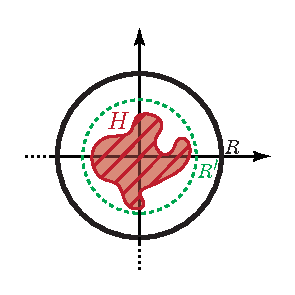
\includegraphics[trim=2cm 0cm 0cm 0cm, clip, scale=0.75]{images/discoconvergenzainsiemeH.pdf}
\end{minipage}\hspace{-7mm}
\begin{minipage}{0.53\textwidth}
	Poiché $H$ è solo \textit{strettamente contenuto} nel disco aperto di convergenza, $\exists R'<R$ tale che si abbia $\overline{H}\subseteq B_{R'}\left(0\right)$, ossia $\abs{z}\leq R',\ \forall z\in H$.\\
	Allora si ha, $\forall n\geq 0$ e $\forall z\in H$
	\begin{equation*}
		\abs{a_nz^n}=\abs{a_n}\abs{z}^n\leq \underbrace{\abs{a_n}\left(R'\right)^n}_{\stackrel{\text{non dipende}}{\text{da }z}}
	\end{equation*}
\end{minipage}\\
	Inoltre, la serie $\displaystyle\sum_{n=0}^{+\infty}c_n=\sum_{n=0}^{+\infty}\abs{a_n}\left(R'\right)^n$ converge in quanto è la convergenza della serie di potenze per il punto $z=R'$, che è interno al disco di convergenza $B_R\left(0\right)$. Applicando il criterio di Weierstrass otteniamo la tesi.
	\item Si ripete la dimostrazione sull'insieme $\overline{B_R\left(0\right)}$ con $R'=R$, considerando che la serie $\displaystyle\sum_{n=0}^{+\infty}\abs{a_n}R^n$ converge per ipotesi sulla convergenza sul bordo.
	\end{enumerate}
\end{demonstration}
\begin{example}\textsc{Serie geometrica.}\\
	Sulla \textit{serie geometrica} $\displaystyle\sum_{n=0}^{+\infty}z^n$ abbiamo già ricavato diverse informazioni: ha raggio di convergenza $R=1$ e \textit{non} c'è convergenza (assoluta) sul bordo. Studiamo ora la convergenza uniforme.
	\begin{itemize}
		\item Converge uniformemente su ogni insieme $H$ tale che $\overline{H}\subsetneqq B_1\left(0\right)$ per il teorema precedente.
		\item Non avendo alcuna convergenza sul bordo, a priori non possiamo dare risultati generali sulla convergenza uniforme sulla base del teorema visto. Tuttavia, possiamo mostrare direttamente - grazie al fatto che la somma parziale e limite della serie geometrica è nota\footnote{Nelle ‘‘Note aggiuntive'', a pagina XXX è possibile trovare maggiori dettagli sulla somma (parziale) della serie geometrica e come ricavarla.} -  che la serie non converge uniformemente sul disco aperto $B_1\left(0\right)$. Infatti
		\begin{align*}
			\sup_{z\in B_1\left(0\right)}\abs{S_n\left(z\right)-S\left(z\right)}&=\sup_{z\in B_1\left(0\right)}\abs{\frac{1-z^{n+1}}{1-z}-\frac{1}{1-z}}=\sup_{z\in B_1\left(0\right)}\abs{\frac{-z^{n+1}}{1-z}}=\\
			&=\sup_{z\in B_1\left(0\right)}\frac{\abs{z}^{n+1}}{\abs{1-z}}=+\infty,\ \forall n\geq 0
		\end{align*}
		da cui
		\begin{equation*}
			\lim_{n\to+\infty}\left(\sup_{z\in B_1\left(0\right)}\abs{S_n\left(z\right)-S\left(z\right)}\right)=+\infty\neq 0
		\end{equation*}
	\end{itemize}
\end{example}
\subsection{Proprietà di regolarità della somma di una serie di potenze}
Sia $\displaystyle\sum_{n=0}^{+\infty}a_nz^n$ una serie di potenze con $R>0$ il raggio di convergenza. Studia la \textbf{funzione somma}\index{funzione!somma}
\begin{equation}
	\funztot{f}{B_R\left(0\right)\subseteq\complexset}{\complexset}{z}{\displaystyle\sum_{n=0}^{+\infty}a_nz^n}
\end{equation}
\begin{proposition}[Proprietà di continuità per la somma di una serie di potenze, caso generale.]~{}\\
	La funzione $f$ è continua su $B_R\left(0\right)$.
\end{proposition}
\begin{attention}
	La convergenza della serie di potenze su $B_R\left(0\right)$ \textit{non} è in generale uniforme, ma sappiamo al più che converge uniformemente su $H$ tale che $\overline{H}\subsetneqq B_R\left(0\right)$, quindi dobbiamo tenere conto di questo fattore nelle dimostrazioni che faremo.
\end{attention}
\begin{demonstration}
	Dobbiamo provare che $f\in\mathcal{C}\left(B_R\left(0\right)\right)$, ossia
	\begin{equation*}
		f\text{ continua in }z_0,\ \forall z_0\in B_R\left(0\right)
	\end{equation*}
	Sia $z_0\in B_R\left(0\right)$ fissato. Per proprietà della metrica, allora $\exists R_0 < R$ tale che $z_0\in B_{R_0}\left(0\right)$. Su $B_{R_0}\left(0\right)$ si ha continuità uniforme e dunque, posto
	\begin{equation*}
		S_n\left(z\right)=\sum_{k=0}^{n}a_kz^k
	\end{equation*}
si ha
\begin{enumerate}
	\item $S_n$ continua su $B_{R_0}\left(0\right)$ perché è un polinomio.
	\item $S_n$ converge uniformemente a $f$ su $B_R\left(0\right)$.
\end{enumerate}
Per il teorema di continuità della funzione limite, $f$ è continua in $B_{R_0}\left(0\right)$ e dunque in $z_0$. 
\end{demonstration}
Questo risultato ci permette di parlare della convergenza sul disco aperto, ma se c'è qualche tipo di convergenza sul bordo, e quindi $f$ è definita anche su di esso, si può estendere la continuità di $f$ fino a tale frontiera? Studiamo due casi.
\begin{corollary}[Proprietà di continuità per la somma di una serie di potenze, caso sul bordo con convergenza assoluta.]~{}\\
	Sia data la serie di potenze $\displaystyle\sum_{n=0}^{+\infty}a_nz^n$ con raggio di convergenza $R>0$. Se la serie converge (assolutamente) su $\partial B_R\left(0\right)$ allora la serie è continua su $\overline{B_R\left(0\right)}$.
\end{corollary}
\begin{demonstration}
	Segue immediatamente ricordando che dalle ipotesi di convergenza assoluta sul bordo, sulla base del teorema \ref{convergenzasottoinsiemeH}, pag. \pageref{convergenzasottoinsiemeH}, vale la convergenza uniforme su $\overline{B_R\left(0\right)}$.
\end{demonstration}
Se invece supponiamo che la serie converga in un punto\footnote{Nel caso di più punti di convergenza $z_0,\ z_1,\ \ldots$, la funzione somma $f$ sarà definita su $B_R\left(0\right)\cup\left\{z_0\right\}\cup\left\{z_1\right\}\cup\ldots$. Qui riportiamo per semplicità il caso di un solo punto, ma i risultati successivi sono opportunamente generalizzabili con più punti di convergenza sul bordo.} $z_0$, cioè $\displaystyle\sum_{n=0}^{+\infty}a_nz_0^n$ converge, possiamo definire la \textbf{funzione somma}\index{funzione!somma} come
\begin{equation}
	\funztot{f}{B_R\left(0\right)\cup\left\{z_0\right\}\subseteq\complexset}{\complexset}{z}{\displaystyle\sum_{n=0}^{+\infty}a_nz^n}
\end{equation}
\textbf{[DISEGNINO Z0 PER TEOREMA DI ABEL]} \\ % TO DO:
La convergenza uniforme di $f$ anche sui punti di convergenza $z_0$ sul bordo ci viene garantita dal \textbf{teorema di Abel}\index{teorema!di Abel}.
\begin{theorema}[Teorema di Abel.]~{}\\
	Sia dato la serie di potenze la serie di potenze $\displaystyle\sum_{n=0}^{+\infty}a_nz^n$ con raggio di convergenza $R>0$. Se $\exists z_0=Re^{i\theta_0}$ tale che $\displaystyle\sum_{n=0}^{+\infty}a_nz_0^n$ converge, allora
	\begin{enumerate}
		\item la serie converge uniformemente sul \textit{segmento}
		\begin{equation}
			\Sigma_0=\left\{z\in\complexset\mid z=re^{i\theta_0},\ r\in\left[0,R\right]\right\}
		\end{equation}
	\item La restrizione di $f$ a $\Sigma_0$ è \textit{continua} su $z_0$, ossia
	\begin{equation}
		\lim_{r\to R}f\left(re^{i\theta_0}\right)=f\left(z_0\right)=\sum_{n=0}^{+\infty}a_nz_0^n
	\end{equation}
	\end{enumerate}
\end{theorema}